\subsection{Related Standards}
Standards are an important part of any engineering design. Standards are employed in order to help ensure interoperability between different components within a design or between different designs. In our design, we will be utilizing a variety of different hardware and communication standards. Specifically, we will be discussing the different standards used to communicate between the microcontroller and different sensors on the node, such as \iic, UART, and SPI. We will also describe the LoRa and LoRaWAN standards, which are used to send data from the nodes to the remote server.

\subsubsection{\iic}
Inter-Integrated Circuit (\iic) is a synchronous, multi-master, multi-slave, serial communication bus. The standard was designed in 1982 by Philips Semiconductor and was originally proprietary and used exclusively by Phillips. The first public specification for \iic  was published in 1992 and it is now used by almost all IC manufacturers. \iic is a popular bus because of how simple it is to use. The protocol specifies the speed of only the upper bus and just two wires that are connected to \Vdd with pull-up resistors are required in order to connect a nearly unlimited number of \iic devices. The two wires used are the serial clock wire (SCL) and the serial data wire (SDA). 

The addressing scheme for \iic specifies the use of a 7-bit address. Each \iic device connected to a bus is required to have a unique address. This can be achieved by have a fixed unique address or a set of \iic addresses that can be selected from to ensure a unique address is used. It should be noted that the address bus does have eight bits total on the bus, however, only bits 7 through 1 are used for the address, while bit 0 is used for indicating the read/write status of the device. A 1 indicates that the master device will read from the slave device. Master devices do not require addresses, since they are the ones generating the clock and they address \iic devices connected to the address bus.

The \iic protocol defines a set of states that the SCL and SDA wires can be in. This defines what the overall state of the \iic bus is in. In the idle state, the SCL and SDA wires are both high. Communication begins when the master device generates the start condition. The start condition is defined when SCL is high and SDA transitions from high to low. The master then sends the address of the slave device it wants to communicate with. The address itself is sent over the SDA line along with a series of high/low pulses on the SCL line, indicating when the SDA line should be read. If the read/write bit of the address is set to 0, the master will begin writing to the slave device, otherwise, if the read/write bit is 1, the next byte will be read from the slave device. Once all bytes have been read or written, the master device will generate the stop condition. The stop condition is defined when SCL is high and SDA SDA transitions from low to high. This puts the bus back into the idle state.

In our design, \iic will be utilized as the communication protocol between the gas sensors and the microcontroller. Using the \iic standard will make it simpler and easier read data from the sensors, as opposed to trying to convert and analyze direct analog inputs.

\begin{figure}
    \centering
    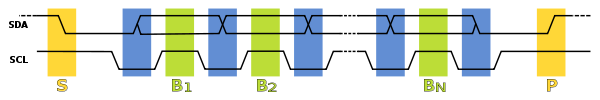
\includegraphics[width=6in]{figures/i2c-protocol.png}
    \caption{A signal graph showing an example of an \iic transmission. Used with permission from \cite{i2c-protocol}.}
    \label{fig:i2c-protocol}
\end{figure}

\subsubsection{SPI}
Serial Peripheral Interface (SPI) is a synchronous serial communication protocol. SPI was created by Motorola in 1979. The protocol operates in full duplex mode, meaning devices connected over SPI can communicate simultaneously. The protocol uses a master/slave architecture. The master device can communicate with multiple slaves.

The signals that each device uses in a SPI setup is slightly different depending on if it is a master or slave device. The signal descriptions are as follows:
\begin{itemize}
    \item SCLK: Serial Clock
    \item MOSI: Master Out Slave In
    \item MISO: Master In Slave Out
    \item CS: Chip Select (sometimes called Slave Select (SS))
\end{itemize}

\begin{figure}
    \centering
    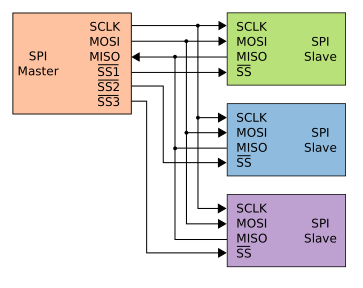
\includegraphics[scale=0.5]{figures/spi-three-slaves.png}
    \caption{An example of the independent slave configuration of SPI. Used with permission from Colin Burnett, under the CC BY-SA 3.0 license.}
    \label{spi-three-slaves}
\end{figure}

The SCLK carries the clock signal and goes from the master to all slave devices. The MOSI signal carries data from the master to each slave. The MISO signal carries data from each slave to the master. The CS signal is used to determine which slave is currently communicating with the master. For the CS signal, there are a few different configurations that are possible. Those configurations are listed as follows:
\begin{itemize}
    \item Independent Slave Configuration: This is the most common configuration used. There is one CS for every slave device connected. An example showing this configuration, is shown in Figure \ref{spi-three-slaves}. This figure also shows how the signals are connected in SPI.
    \item Daisy Chain Configuration: In this configuration, there is a signal CS signal going from the master to each slave device. This configuration also somewhat changes how the MOSI and MISO signals of slave devices are used. The MISO signal goes from one slave to the MOSI pin of another slave, this is repeated until the last slave in the chain connects it's MISO pin back to the master's MISO pin.
\end{itemize}

The process of SPI communication occurs during clock cycles. SPI communication begins by the master configuring the clock and then selecting the slave device which is set to low on the CS line. Then, during each clock cycle, data transmission occurs over the MOSI and MISO lines between the master and slave. The master reads a word of data, usually 8-bits, over the MISO line and the master transmits a word of data over the MOSI line. This exchange of words can occur multiple times. Once the final word has been transmitted between the master and currently selected slave, on the next clock cycle the next slave is selected and the process repeats.

\subsubsection{UART}
Universal Asynchronous Receiver Transmitter (UART) is one of the most popular and widely-used communication protocols. UART is relatively simple protocol, requiring only two wires to function. Each UART device utilizes two pins, an receiving (RX) pin and a transmitting (TX) pin. In a situation where two UART devices are connected with one another, the first device's RX pin will be connected to the second devices TX pin and the first device's TX pin will be connected to the other devices RX pin. Another requirement of UART is that the baud rate must be the same for two UART devices that are connected to each other.

The UART protocol defines that data is sent in a packet structure (Figure \ref{fig:uart-data-packet}). A UART packet includes a start bit, the data frame, a parity bit, and one to two stop bits. In the idle state, the TX line remains high. Communication begins when the TX line transitions from high to low for one clock cycle. After the start bit, the data frame, which contains the actual data being sent, is transmitted. This is performed by setting the TX wire to high when a 1 is transmitted and to low when a 0 is transmitted. This wire is sampled by the receiving UART device at the predetermined baudrate. Due to the fact that the parity bit is optional, the data frame may be eight or nine bits long. After the last data bit is transmitted, the parity bit is transmitted. This bit used to tell if any data has been altered during the transmission process. The parity bit is calculated by summing the 1's and 0's of the data frame and then, depending on whether or not the sum is even or odd, the parity bit is set to 0 or 1 respectively. Finally, the stop bit is transmitted to indicate the end of the packet. This is done when the TX line transitions from low to high for one or two clock cycles.

\begin{figure}
    \centering
    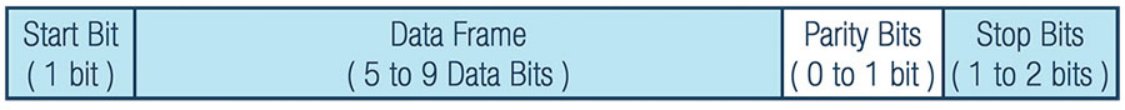
\includegraphics[width=6in]{figures/uart-data-packet.png}
    \caption{The structure of the UART data packet.}
    \label{fig:uart-data-packet}
\end{figure}

\subsubsection{USB}
Universal Serial Bus (USB) is an industry standard the creates specifications for physical connectors and communication protocols for those connectors. The goal of the USB standard is to simplify and improve the interface between personal computers and peripheral devices. The different communication protocols that uSB specifies include USB 1.0, USB 1.1, USB 2.0, USB 3.0, USB 3.1, USB 3.2, and USB4. This list of communication protocols dates back to the inception of USB in 1996. Today, only USB 3.0 and up are common on new devices. The different connectors include Type A, B, and C. The Type C connector is the most modern connector and supports the newest communication protocols, reaching a maximum data rate of 40 Gbps. However, many new devices still support the Type A connector. 

\subsubsection{LoRa}
LoRa (Long Range) is a proprietary, wireless modulation technique derived from chirp spread spectrum (CSS) technology. LoRa is was developed and patented by Semtech. LoRa only covers the physical layer. An additional protocol is necessary in order to specify the upper layers required for a functioning communication system. LoRaWAN is the one of the most widely used protocols to fulfill this purpose and will be discussed later in this section.

One of the reasons for choosing LoRa over other communication standards, such as WiFi or cellular, is due to where it stands in relation to bandwidth, range, and power. Technologies such as Bluetooth and WiFi are considered high bandwidth, but low range. Cellular technology is high range and can be high bandwidth, but a major drawback is the high operating power required. In contrast, LoRa is low power, high range, and can operate in the license-free frequency band in the United States, as well as in other countries. Figure \ref{fig:lora-range-bandwidth} shows a comparison between these different types of technology.

\begin{figure}
    \centering
    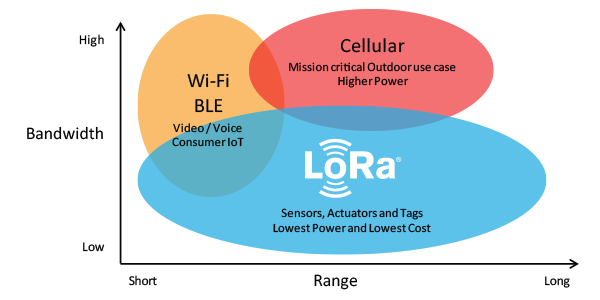
\includegraphics[width=6in]{figures/lora-range-bandwidth.png}
    \caption{A range-bandwidth comparison between WiFi and Bluetooth LE, cellular, and LoRa. Used with permission, according to the terms and conditions.}
    \label{fig:lora-range-bandwidth}
\end{figure}


In order to explain how LoRa functions, we must first give a brief overview of CSS. CSS is a communication technique that utilizes its entire allocated bandwidth to broadcast a signal. It uses wideband linear frequency modulated chirp pulses to encode information. A chirp is simply a signal whose frequency changes over time according to specific, time-varying function \cite{ieee-std-chirp}. In the case of LoRa, the frequency band that is used is the license-free sub-GHz radio frequency that varies by region. For example, in the United States the license-free radio frequency band is 920 MHz to 928 MHz. The modulation technique that LoRa uses is derived from CSS. It functions by representing each bit of data in a payload as multiple chirps. LoRa defines a term known as spreading factor ($SF$) to refer to the number of symbols sent per bit of information. Since multiple chirps are used to represent a single bit of data, spreading factor is also the relationship between the nominal symbol rate and the nominal chirp rate. The creates a discrete modulation where the $M=2^{SF}$ possible waveforms at the output of the modulator are chirp modulated signals over the frequency interval $(f_0 - B/2, f_0 + B/2)$, where B is the bandwidth. There are $M$ initial frequencies \cite{ieee-lora-modulation}.

LoRa supports the ability to trade fixed sensitivity within a fixed channel bandwidth for data rate. It does this by modifying the $SF$ parameter. A higher $SF$ has the benefit of giving the receiver more chances to sample the signal power, providing better sensitivity. However, the drawback to a higher $SF$ value is the greater transmission time and thus higher energy consumption, which is clearly a negative for the low-power applications that LoRa devices are typically used in. Understandably, a lower $SF$ value results in more chirps per second, meaning worse sensitivity for the receiver. However, the benefit is the lower power consumption \cite{ttn-spreading-factor}.

Another parameter of LoRa is the transmission power. Depending on the region the specific LoRa module is targeted for, the supported range of transmission power ranges from 2 dBm to 14 dBm in certain areas in Europe and Asia to as high as 20 dBm in some parts of Europe and all of North America. This means LoRa can support a transmission distance of up to 10 miles in ideal conditions e.g. line of sight.

\subsubsection{LoRaWAN}
LoRaWAN (Long Range Wide Area Network) is a protocol that defines the network portion of a LoRa stack. There are many different protocols that exist to fulfill the same role as LoRaWAN, however, LoRaWAN is public and is widely supported by many different hardware vendors. In fact, the LoRa Alliance was created in 2015 to support the development of LoRaWAN and ensure the standardization of all products and technologies utilizing LoRaWAN. The LoRa Alliance is composed of many different technology companies and organization, including high-profile members such as IBM and Cisco.

LoRaWAN is often referred to as using a "star of stars" network technology. What this means is that LoRaWAN consists of a collection of gateways which communicate with a central i.e. a classic star network topology. On top of this, each gateway communicates with a collection of end-devices, often referred to as nodes as they are in our design, creating a star sub-network topology. Figure \ref{lorawan-network-stack} shows the layout LoRaWAN's network topology. LoRaWAN specifies that the gateways communicate with the server using IP packets. This means that the gateways are simply acting as a bridge between the RF signals coming from the end-devices and the IP packets being transmitted to the central server. In the context of the OSI model, LoRaWAN operates in between the physical LoRa standard and the application layer \cite{lora-alliance}.

\begin{figure}
    \centering
    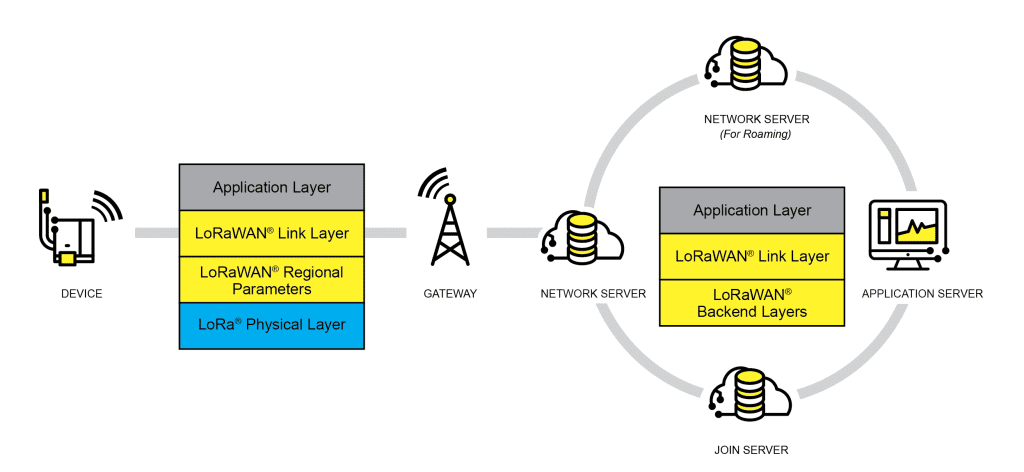
\includegraphics[width=6in]{figures/lorawan-stack.png}
    \caption{The LoRaWAN network topology.}
    \label{lorawan-network-stack}
\end{figure}

The LoRaWAN specification specifies three possible different end-device types, which are summarized in Table \ref{tab:lorawan-classes} and described in more detail below:

\begin{itemize}
    \item \textbf{Class A} devices are described as lowest power, bidirectional end-devices. For an end-device to compliant with the LoRaWAN specification, it must be able to function as a Class A device. Class A devices always initiate communication with the central server and can do this asynchronously. Every time a Class A device begins an uplink transmission, it must be followed by two downlink transmissions. This allows the server to send follow-up communication, hence the bidirectional description of the class. The LoRaWAN specification states that the central server must buffer downlink communication until the next uplink transmission from the end-device. Once an end-device has finished sending and receiving transmissions, it can enter a low-power state that it can define.
    
    
    \item \textbf{Class B} devices are described bidirectional end-devices with deterministic downlink latency. Class B devices still initiate communication with the central server, however, they initiate this communication during scheduled, periodic intervals. This means that the central server can send a downlink transmission predictably. This means that the end-devices will consume additional power. This transmission latency can be configured up to a maximum of 128 seconds.
    
    
    \item \textbf{Class C} devices are described as bidirectional end-devices with the lowest possible downlink latency. This lowest possible downlink latency is achieved because the end-device is simply ready to receive at all times. The only time the end-device is not ready to receive is when it is transmitting data back to the central server. Due to the large power consumption, the ideal situation for Class C device would be for it to be connected to external power. For battery operated applications, it is possible to have a device temporarily switch between Class A and Class C.
\end{itemize}


\begin{table}[]
\centering
\begin{tabular}{|c|c|c|c|}
\hline
Class & Latency & Power Consumption & Transmission Pattern \\\hline
\hline
Class A & Highest & Lowest & End-device initiated (asynchronous) \\\hline
Class B & Middle & Middle & End-device initiated (synchronous) \\\hline
Class C & Lowest & Highest & Continuous \\\hline
\end{tabular}
\caption{A summary of the three different LoRaWAN end-device classes.}
\label{tab:lorawan-classes}
\end{table}

LoRaWAN also specifies a parameter known as data rate. The data rate parameter controls the relationship between communication range and message duration. In addition, due to how spread-spectrum technology functions, end-devices communicating with different data rates do not interfere with one another. This effectively increases the capacity of each gateway by essentially creating multiple separate channels which are delineated by the data rate parameter. Taking advantage of this information, LoRaWAN specifies the creation of a scheme known as Adaptive Data Rate (ADR). The ADR scheme is defined by having the central server manage the data rate parameter and transmission power for each end-device. This can allow the central server to optimize battery life for end-devices and optimize the capacity of the network. The possible values for the data rate range from 0.3 Kbps to 50 Kbps.

The LoRaWAN specification also takes into account security. The specification details two layers of security. This is done via the inclusion of a 128-bit AES Network Session Key, which is shared between an end-device and the network server, and a 128-bit AES Application Session Key, which is shared between the end-device and network server at the application level. This results in the benefit of having authentication and verification of packets traveling from end-devices to the central server and end-to-end packet encryption from the end-device to the end application server. These features make it possible to have shared networks without the owner of the network being able to view packets.
